\documentclass[border=4pt,12pt]{standalone}
% House style for redrawn exam diagrams (diagram-v4: 0.4pt lines, filled -latex arrows, fine dashes; stipple and hatching drawn as real dots/lines (no PDF/SVG patterns, so they render in every browser and at any scale); transparent background). Every figure \input's this.
\usepackage{amsmath,amssymb}
\usepackage{txfonts}
\usepackage{pdfrender,xcolor}
% \halo{text}: label on shading. The shading stops just around each letter's outline (a thin knock-out that follows the
% glyphs, like the papers' typesetting), never a box. Owner: "I don't want a box around the text".
\newcommand{\halo}[1]{\leavevmode\rlap{\pdfrender{TextRenderingMode=2,LineWidth=2.2pt,LineJoinStyle=1,StrokeColor=white,FillColor=white}#1}#1}
\usepackage{tikz,pgfplots}
\pgfplotsset{compat=1.18}
\usetikzlibrary{arrows.meta,calc,angles,quotes,patterns,patterns.meta,intersections,positioning,decorations.markings,shapes.geometric}
% Stipple and hatching are drawn as actual dots / lines clipped to the region (path picture), NOT as pattern fills:
% SVG <pattern> fills vanish or blur when browsers scale the image, so the owner could not see the shading.
% Each dot is a 0.72pt square (keeps SVGs small; reads as a dot at print size). Dots sit on one global staggered grid, so neighbouring regions line up.
\makeatletter
\newdimen\ex@x \newdimen\ex@y \newdimen\ex@xa \newdimen\ex@ya \newdimen\ex@xb \newdimen\ex@yb \newcount\ex@row
\def\exam@stipplecolor{black!75}\def\exam@dotr{0.42pt}\def\exam@dotgap{2.5}
\def\ex@rowdots{\ifdim\ex@x<\ex@xb \pgfpathrectangle{\pgfqpoint{\dimexpr\ex@x-0.36pt\relax}{\dimexpr\ex@y-0.36pt\relax}}{\pgfqpoint{0.72pt}{0.72pt}}\advance\ex@x by \exam@dotgap pt\relax\expandafter\ex@rowdots\fi}
\def\exam@stipple{%
  \pgftransformreset% dots are sized in real points even inside scaled pictures
  \pgfpointanchor{path picture bounding box}{south west}\ex@xa=\pgf@x \ex@ya=\pgf@y
  \pgfpointanchor{path picture bounding box}{north east}\ex@xb=\pgf@x \ex@yb=\pgf@y
  \pgfsetfillcolor{\exam@stipplecolor}\pgfmathsetmacro\ex@h{\exam@dotgap/2}%
  \pgfmathtruncatemacro\ex@r{floor(\ex@ya/\ex@h)-1}\ex@row=\ex@r\relax
  \ex@y=\ex@r\dimexpr\ex@h pt\relax
  \loop\ifdim\ex@y<\ex@yb
    \pgfmathtruncatemacro\ex@c{floor(\ex@xa/\exam@dotgap)-1}\ex@x=\ex@c\dimexpr\exam@dotgap pt\relax
    \ifodd\ex@row \advance\ex@x by \ex@h pt\fi
    \ex@rowdots
    \advance\ex@y by \ex@h pt \advance\ex@row by 1
    \ifnum\numexpr\ex@row-(\ex@row/4)*4\relax=0 \pgfusepath{fill}\fi% flush every 4 rows: bounded TeX memory, few clip copies in the SVG
  \repeat\pgfusepath{fill}}
\newdimen\ex@d
\def\exam@hatch#1{% #1 = 1 for /, -1 for \ ; lines 45 degrees, 3pt apart
  \pgftransformreset
  \pgfpointanchor{path picture bounding box}{south west}\ex@xa=\pgf@x \ex@ya=\pgf@y
  \pgfpointanchor{path picture bounding box}{north east}\ex@xb=\pgf@x \ex@yb=\pgf@y
  \ex@d=\dimexpr\ex@yb-\ex@ya\relax \ex@x=\dimexpr\ex@xa-\ex@d\relax
  \loop\ifdim\ex@x<\ex@xb
    \ifnum#1>0 \pgfpathmoveto{\pgfqpoint{\ex@x}{\ex@ya}}\pgfpathlineto{\pgfqpoint{\dimexpr\ex@x+\ex@d\relax}{\ex@yb}}%
    \else \pgfpathmoveto{\pgfqpoint{\ex@x}{\ex@yb}}\pgfpathlineto{\pgfqpoint{\dimexpr\ex@x+\ex@d\relax}{\ex@ya}}\fi
    \advance\ex@x by 4.24pt
  \repeat
  \pgfsetlinewidth{0.4pt}\pgfsetstrokecolor{black}\pgfusepath{stroke}}
\def\examstipple{\exam@stipple}\def\examhatch{\exam@hatch}\def\examsetstipplecolor#1{\def\exam@stipplecolor{#1}}\def\examsetdotgap#1{\def\exam@dotgap{#1}}
\makeatother
% (legacy pattern kept for old files)
% staggered stipple like the NESA papers' dotted shading
\pgfdeclarepatternformonly{exam stipple}{\pgfpointorigin}{\pgfqpoint{2.2pt}{2.2pt}}{\pgfqpoint{2.2pt}{2.2pt}}{%
  \pgfpathcircle{\pgfqpoint{0.55pt}{0.55pt}}{0.42pt}\pgfpathcircle{\pgfqpoint{1.65pt}{1.65pt}}{0.42pt}\pgfusepath{fill}}
\tikzset{
  every picture/.style={line width=0.6pt, >={Latex[length=2mm,width=1.3mm]}},
  curve/.style={line width=0.6pt},
  open arrow/.style={-{Latex[length=2mm,width=1.3mm]}},  % owner: filled -latex heads everywhere, no open chevrons
  aux/.style={dash pattern=on 2pt off 1.5pt, line width=0.6pt},
  shade/.code={\def\exA{#1}\def\exB{none}\ifx\exA\exB\else\pgfkeysalso{fill=black!18}\fi},
  shade/.default=on,
  shade dots/.style={fill=none, path picture={\examstipple}},
  stipple color/.code={\examsetstipplecolor{#1}},
  stipple gap/.code={\examsetdotgap{#1}},
  shade dense dots/.style={fill=none, stipple gap=1.6, path picture={\examstipple}},
  shade hatch/.style={fill=none, path picture={\examhatch{1}}},
  shade hatch reverse/.style={fill=none, path picture={\examhatch{-1}}},
  shade solid/.style={fill=black},
  pt/.style={circle, fill, inner sep=1.1pt},
  open pt/.style={circle, draw, fill=white, inner sep=1.1pt},
}
\pgfplotsset{
  exam axes/.style={axis lines=middle, axis line style={->}, xlabel={$x$}, ylabel={$y$},
    xlabel style={anchor=west}, ylabel style={anchor=south}, tick label style={font=\small},
    every axis plot/.append style={line width=0.6pt, black}, samples=200, clip=false,
    enlargelimits=false, axis on top},
}

\begin{document}
% crop pixel units (y down); origin (112,452.5); curves traced from the crop (desmooth)
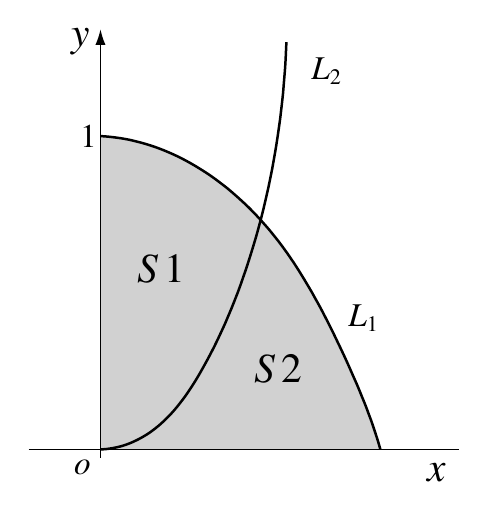
\begin{tikzpicture}[x=0.0127cm,y=-0.0127cm, every node/.style={inner sep=0pt}]
  \fill[shade] plot[smooth] coordinates {(112,139) (119.1,139.5) (126.2,140.3) (133.3,141.3) (140.4,142.6) (147.3,144.2) (154.2,146) (161.2,148.1) (168,150.4) (174.8,153) (181.5,155.8) (188.1,158.8) (194.7,162.1) (201,165.5) (207.4,169.2) (213.7,173.1) (219.9,177.1) (225.9,181.3) (231.9,185.8) (237.8,190.3) (243.5,195.1) (249.1,200) (254.6,205) (260.1,210.2) (265.3,215.5) (270.5,221) (275.5,226.6) (280.4,232.2) (285.2,238.1) (289.9,244) (294.4,250) (298.8,256.1) (303.2,262.5) (307.4,268.8) (311.5,275.3) (315.5,281.8) (319.5,288.5) (323.5,295.3) (327.2,302) (331,308.8) (334.7,315.8) (338.3,322.8) (341.8,329.7) (345.3,336.8) (348.7,343.9) (352.1,351) (355.5,358.2) (358.8,365.4) (362,372.6) (365.2,379.9) (368.4,387.1) (371.4,394.3) (374.4,401.7) (377.3,408.8) (380,416.1) (382.7,423.3) (385.2,430.6) (387.6,437.9) (389.9,445.1) (392,452.5)} -- (112,452.5) -- cycle;
  \draw (40,452.5) -- (471,452.5);
  \draw[->] (112,461) -- (112,32);
  \draw[line width=0.9pt] plot[smooth] coordinates {(112,139) (119.1,139.5) (126.2,140.3) (133.3,141.3) (140.4,142.6) (147.3,144.2) (154.2,146) (161.2,148.1) (168,150.4) (174.8,153) (181.5,155.8) (188.1,158.8) (194.7,162.1) (201,165.5) (207.4,169.2) (213.7,173.1) (219.9,177.1) (225.9,181.3) (231.9,185.8) (237.8,190.3) (243.5,195.1) (249.1,200) (254.6,205) (260.1,210.2) (265.3,215.5) (270.5,221) (275.5,226.6) (280.4,232.2) (285.2,238.1) (289.9,244) (294.4,250) (298.8,256.1) (303.2,262.5) (307.4,268.8) (311.5,275.3) (315.5,281.8) (319.5,288.5) (323.5,295.3) (327.2,302) (331,308.8) (334.7,315.8) (338.3,322.8) (341.8,329.7) (345.3,336.8) (348.7,343.9) (352.1,351) (355.5,358.2) (358.8,365.4) (362,372.6) (365.2,379.9) (368.4,387.1) (371.4,394.3) (374.4,401.7) (377.3,408.8) (380,416.1) (382.7,423.3) (385.2,430.6) (387.6,437.9) (389.9,445.1) (392,452.5)};
  \draw[line width=0.9pt] plot[smooth] coordinates {(112,452.5) (118.5,452) (125,451) (131.4,449.6) (137.6,447.7) (143.7,445.3) (149.8,442.4) (155.6,439.2) (161.4,435.5) (166.9,431.4) (172.3,426.9) (177.5,422) (182.6,416.8) (187.5,411.2) (192.2,405.3) (196.8,399.2) (201.3,392.6) (205.6,386) (209.8,379.1) (213.9,371.9) (217.9,364.7) (221.9,357.2) (225.7,349.8) (229.4,342.2) (232.9,334.7) (236.4,327.1) (239.7,319.3) (243,311.5) (246.1,303.7) (249.2,295.8) (252.1,287.9) (254.9,279.8) (257.7,271.8) (260.3,263.7) (262.9,255.5) (265.4,247.3) (267.8,239.2) (270.1,230.9) (272.3,222.7) (274.4,214.5) (276.4,206.1) (278.3,197.8) (280.2,189.4) (281.9,181) (283.6,172.7) (285.1,164.3) (286.6,155.8) (288,147.4) (289.3,138.9) (290.5,130.5) (291.7,122) (292.7,113.5) (293.7,104.9) (294.6,96.38) (295.3,87.83) (296,79.27) (296.7,70.71) (297.2,62.26) (297.6,53.69) (298,45)};
  \node[font=\fontsize{15}{17}\selectfont] at (92,44) {$y$};
  \node[font=\fontsize{12}{14}\selectfont] at (100,139) {1};
  \node[font=\fontsize{12}{14}\selectfont] at (94,470) {$o$};
  \node[font=\fontsize{15}{17}\selectfont] at (447,476) {$x$};
  \node[font=\fontsize{15}{17}\selectfont] at (173,272) {$S1$};
  \node[font=\fontsize{15}{17}\selectfont] at (290,372) {$S2$};
  \node[font=\fontsize{12}{14}\selectfont] at (375,321) {$L_1$};
  \node[font=\fontsize{12}{14}\selectfont] at (338,74) {$L_2$};
\end{tikzpicture}
\end{document}
